\chapter{Measures of Momentum}
%

\section{Stochastic Oscillator}
%
The basis for the stochastic oscillator \eqref{eq:stochasticOscillator} stems from considerable historical evidence of prices closing near their high during upward trends, and prices closing near their low in downward trends.  The indicator is termed and oscillator because it fluctuates between two extrema.  The ratio is a percentage how close the current price is to the average high, relative to the range between the average high and low.
%
\begin{flalign}
\label{eq:stochasticOscillator}
\%K_{\ell,n} &= 100 \cdot (\frac{c_{n}-l_{\ell,n}}{h_{\ell,n}-l_{\ell,n}}) \\
{} & \mbox{where} \nonumber \\
{} & c_{\ell,n} \mbox{ is the closing price over the interval of $\ell$ } \nonumber \\
{} & h_{\ell,n} \mbox{ is the hight price over the interval of $\ell$ } \nonumber \\
{} & l_{\ell,n} \mbox{ is the low price over the interval of $\ell$ } \nonumber \\
{} & \mbox{with typical values $\ell$ = 14 days } \nonumber \\
\end{flalign}
\captionof{figure}{Stochastic Oscillator}
%
\par
A trigger line, given by equation \eqref{eq:stochasticOscillatorSignal} is used to determine when a price inflection will occur.  This trigger line is a three-period moving average of the stochastic oscillator.  It is estimated that an inflection will occur when these lines cross.
\par
%
\begin{flalign}
\label{eq:stochasticOscillatorSignal}
\%D = SMA_{N=3\ell}\{\%K\}
\end{flalign}
\captionof{figure}{Stochastic Oscillator Signal Line}
%
The figure below shows LMT in 2009 trading between \$57.11 and \$86.76 for the year.  The \%K and \%R lines for the stochastic oscillator are shown below, giving the same buy indicator during the upward trend 
%
\begin{figure}[ht]\centering
\label{fig:stochasticOscillator}
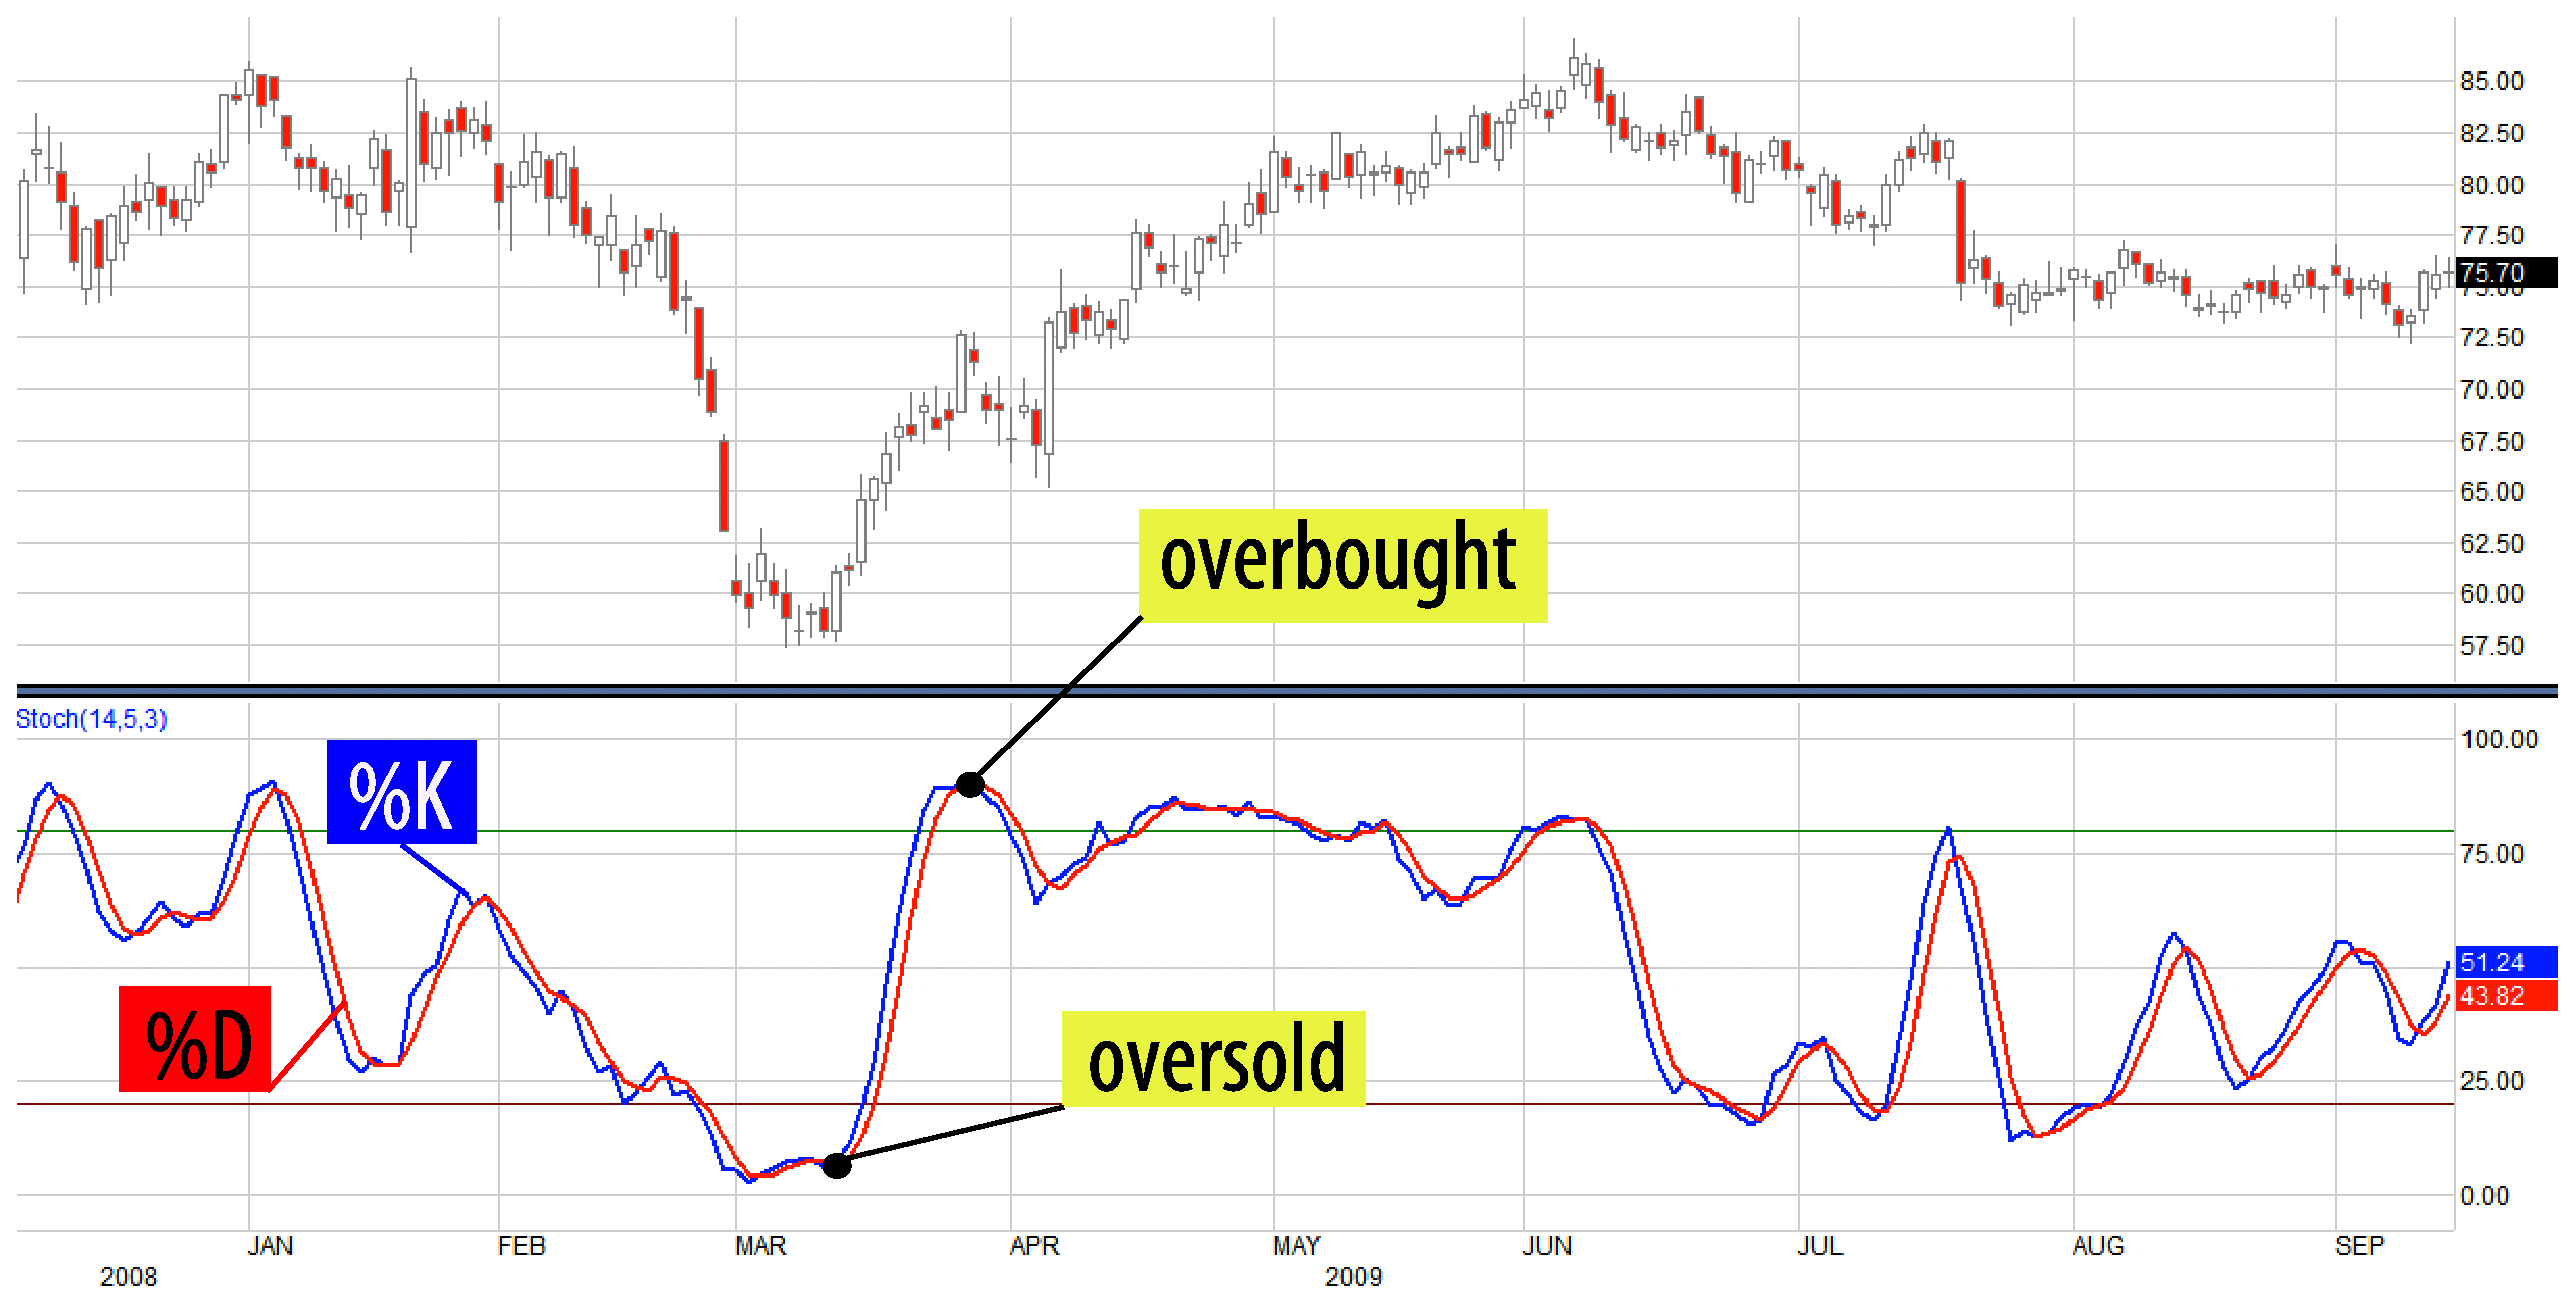
\includegraphics[width=1\textwidth]{figures/Stochastic-LMT-1.eps}
\caption{$\mbox{Stochastic Oscillator} LMT \approx 2009$}
\end{figure}
%
\subsection{Example Revisited - Comparison of Stochastic Oscillator to MACD}
%
Consider LMT around 12-Mar-09 as an example of the stochastic oscillator outperforming the MACD.  Although both indicators agree to enter the trade on this date, the stochastic oscillator triggers to sell at the local maxima on 03-Mar-09 at \$72.69 per share.  The MACD lags the signal, and triggers to sell on 03-Apr-09 at \$67.39 per share, for a differential of $-\$5.30$ per share.  This is illustrated in the figure below (Fig.~\ref{stochasticMACD}) with price signal (top chart), the stocastic oscillator (middle chart) and the MACD (bottom chart).
%
\begin{figure}[ht]\centering
\label{stochasticMACD}
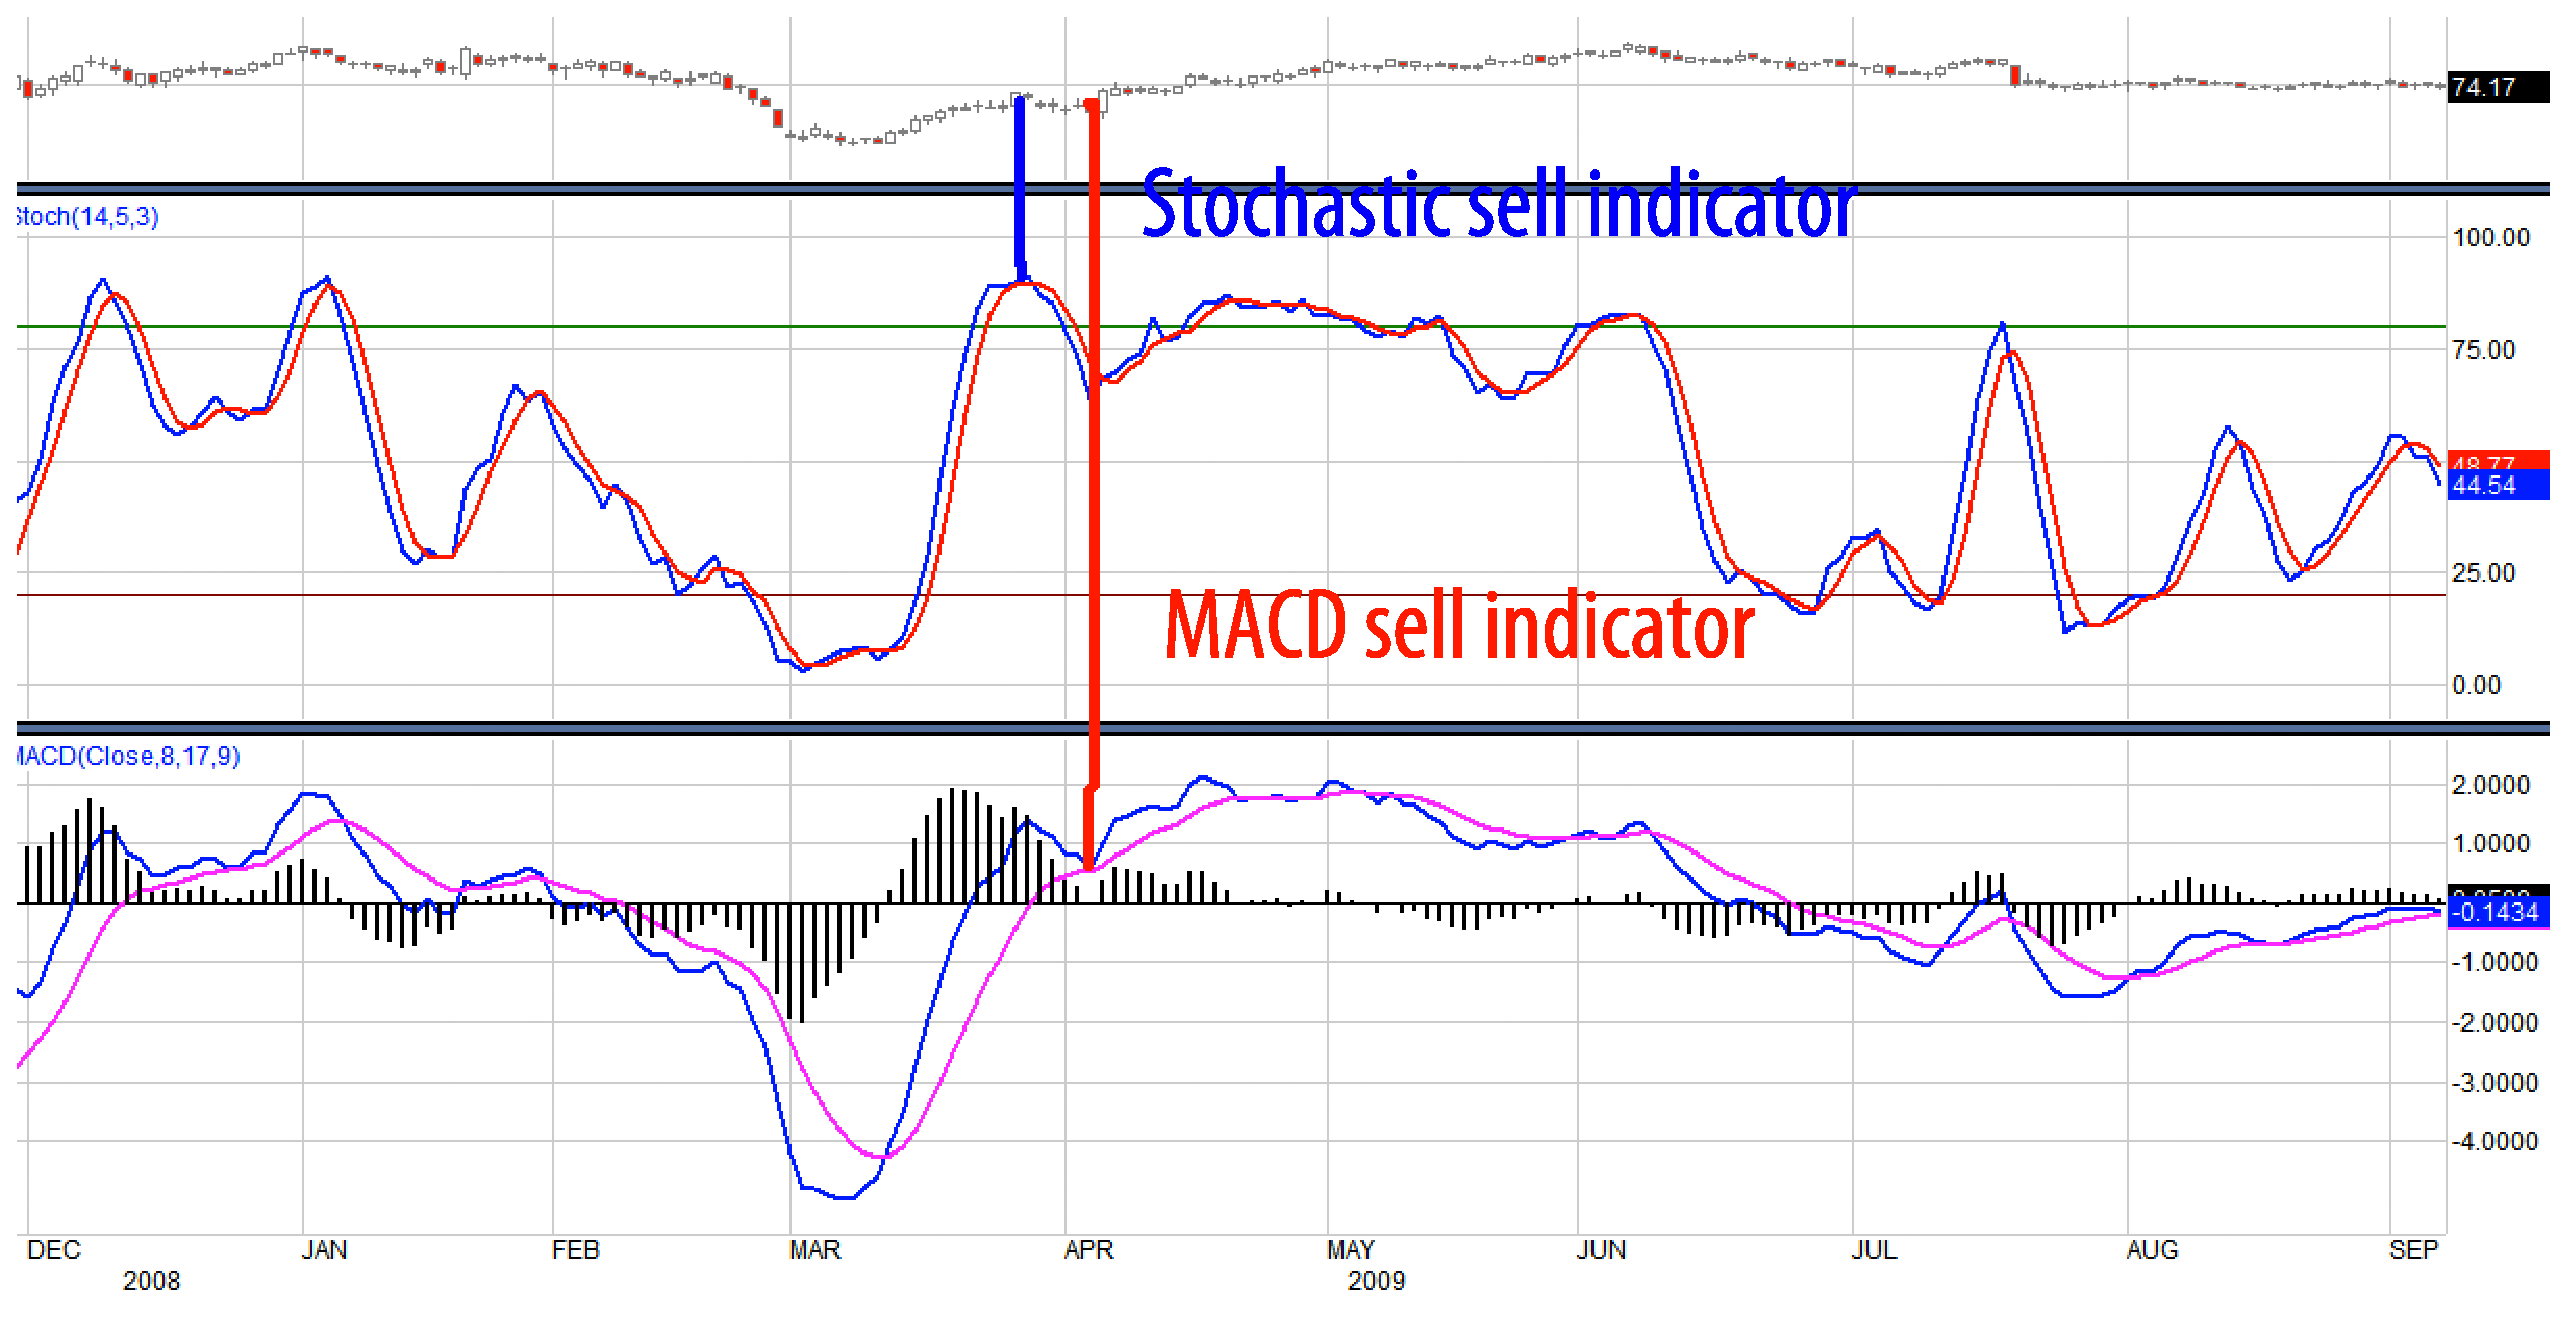
\includegraphics[width=1\textwidth]{figures/Stochastic-MACD-LMT-1.eps}
\caption{$MACD\{c_{LMT \approx 2009}\} \mbox{ and } \%K_{LMT \approx 2009}$}
\end{figure}
%
\section{Williams \%R}
%
The williams \%R \eqref{eq:williamsR} is similar to the stochastic oscillator, but is designed with a negative scale.  The oscillator stays in a range of $[0,-100]$.  When the williams \%R raises above -20 the stock is beleived to be overbought, and when the price drops below -80 it is beleived to be oversold \cite{Wikipedia:WilliamsR}.
%
\begin{flalign}
\label{eq:williamsR}
\%R_{\ell,n} &= 100 \cdot (\frac{c_{n}-h_{\ell,n}}{h_{\ell,n}-l_{\ell,n}}) \\
{} & \mbox{where} \nonumber \\
{} & c_{\ell,n} \mbox{ is the closing price over the interval of $\ell$ } \nonumber \\
{} & h_{\ell,n} \mbox{ is the hight price over the interval of $\ell$ } \nonumber \\
{} & l_{\ell,n} \mbox{ is the low price over the interval of $\ell$ } \nonumber \\
{} & \mbox{with typical values $\ell$ = 10 days } \nonumber \\
\end{flalign}
\captionof{figure}{Williams \%R}
%

\section{Chaikin Money Flow}
%
The Chaikin Money Flow (CMF) is an indicator based on the cumulative accumulation and distribution of a stock, thus taking volume into account.  Positive values reflect accumulation in the market, and negative values reflect distribution.  The extent and strenght of the accumulation/distibution is reflected by the duration (that it is positive/negative) and magnitude, respectively \cite{Investopedia:CMF}.
\par
To compute the CMF, the day's close of taken as a percentage of the range, known as the close location value (CLV) Eq.~\eqref{eq:CLV}.  This percentage is cumulatively added to the volume as a measure of the accumulationd/distribution Eq.~\eqref{eq:AD} \cite{Wikipedia:AccumulationDistribution}.
%
\begin{equation}
\label{eq:CLV}
CLV_{n}=\frac{(c_{n}-l_{n})-(h_{n}-c{n})}{h_{n}-l_{n}}
\end{equation}
\captionof{figure}{Close Location Value}
%
\begin{flalign}
\label{eq:AD}
AD_{n}&=AD_{n-1}+V_{n}CLV_{n} \\
{} & \mbox{where V is the volume in shares } \nonumber \\
\end{flalign}
\captionof{figure}{Accumulation/Distribution Index}
%
\begin{flalign}
\label{eq:CMF}
CMF_{n}&=EMA_{N_{1}}\{AD_{n}\}-EMA_{N_{2}\{AD_{n}\}} \\
{} & \mbox{with typical values $N_{1}=3$ and $N_{2}=10$ } \nonumber \\
\end{flalign}
\captionof{figure}{Chaikin Money Flow}
%
The Chaikin Money Flow is subject to failure during price breakouts and gaps, as the market deviates from the precedented buying and selling pressures \cite{Investopedia:CMF}.
%
\begin{figure}[ht]\centering
\label{CMF}
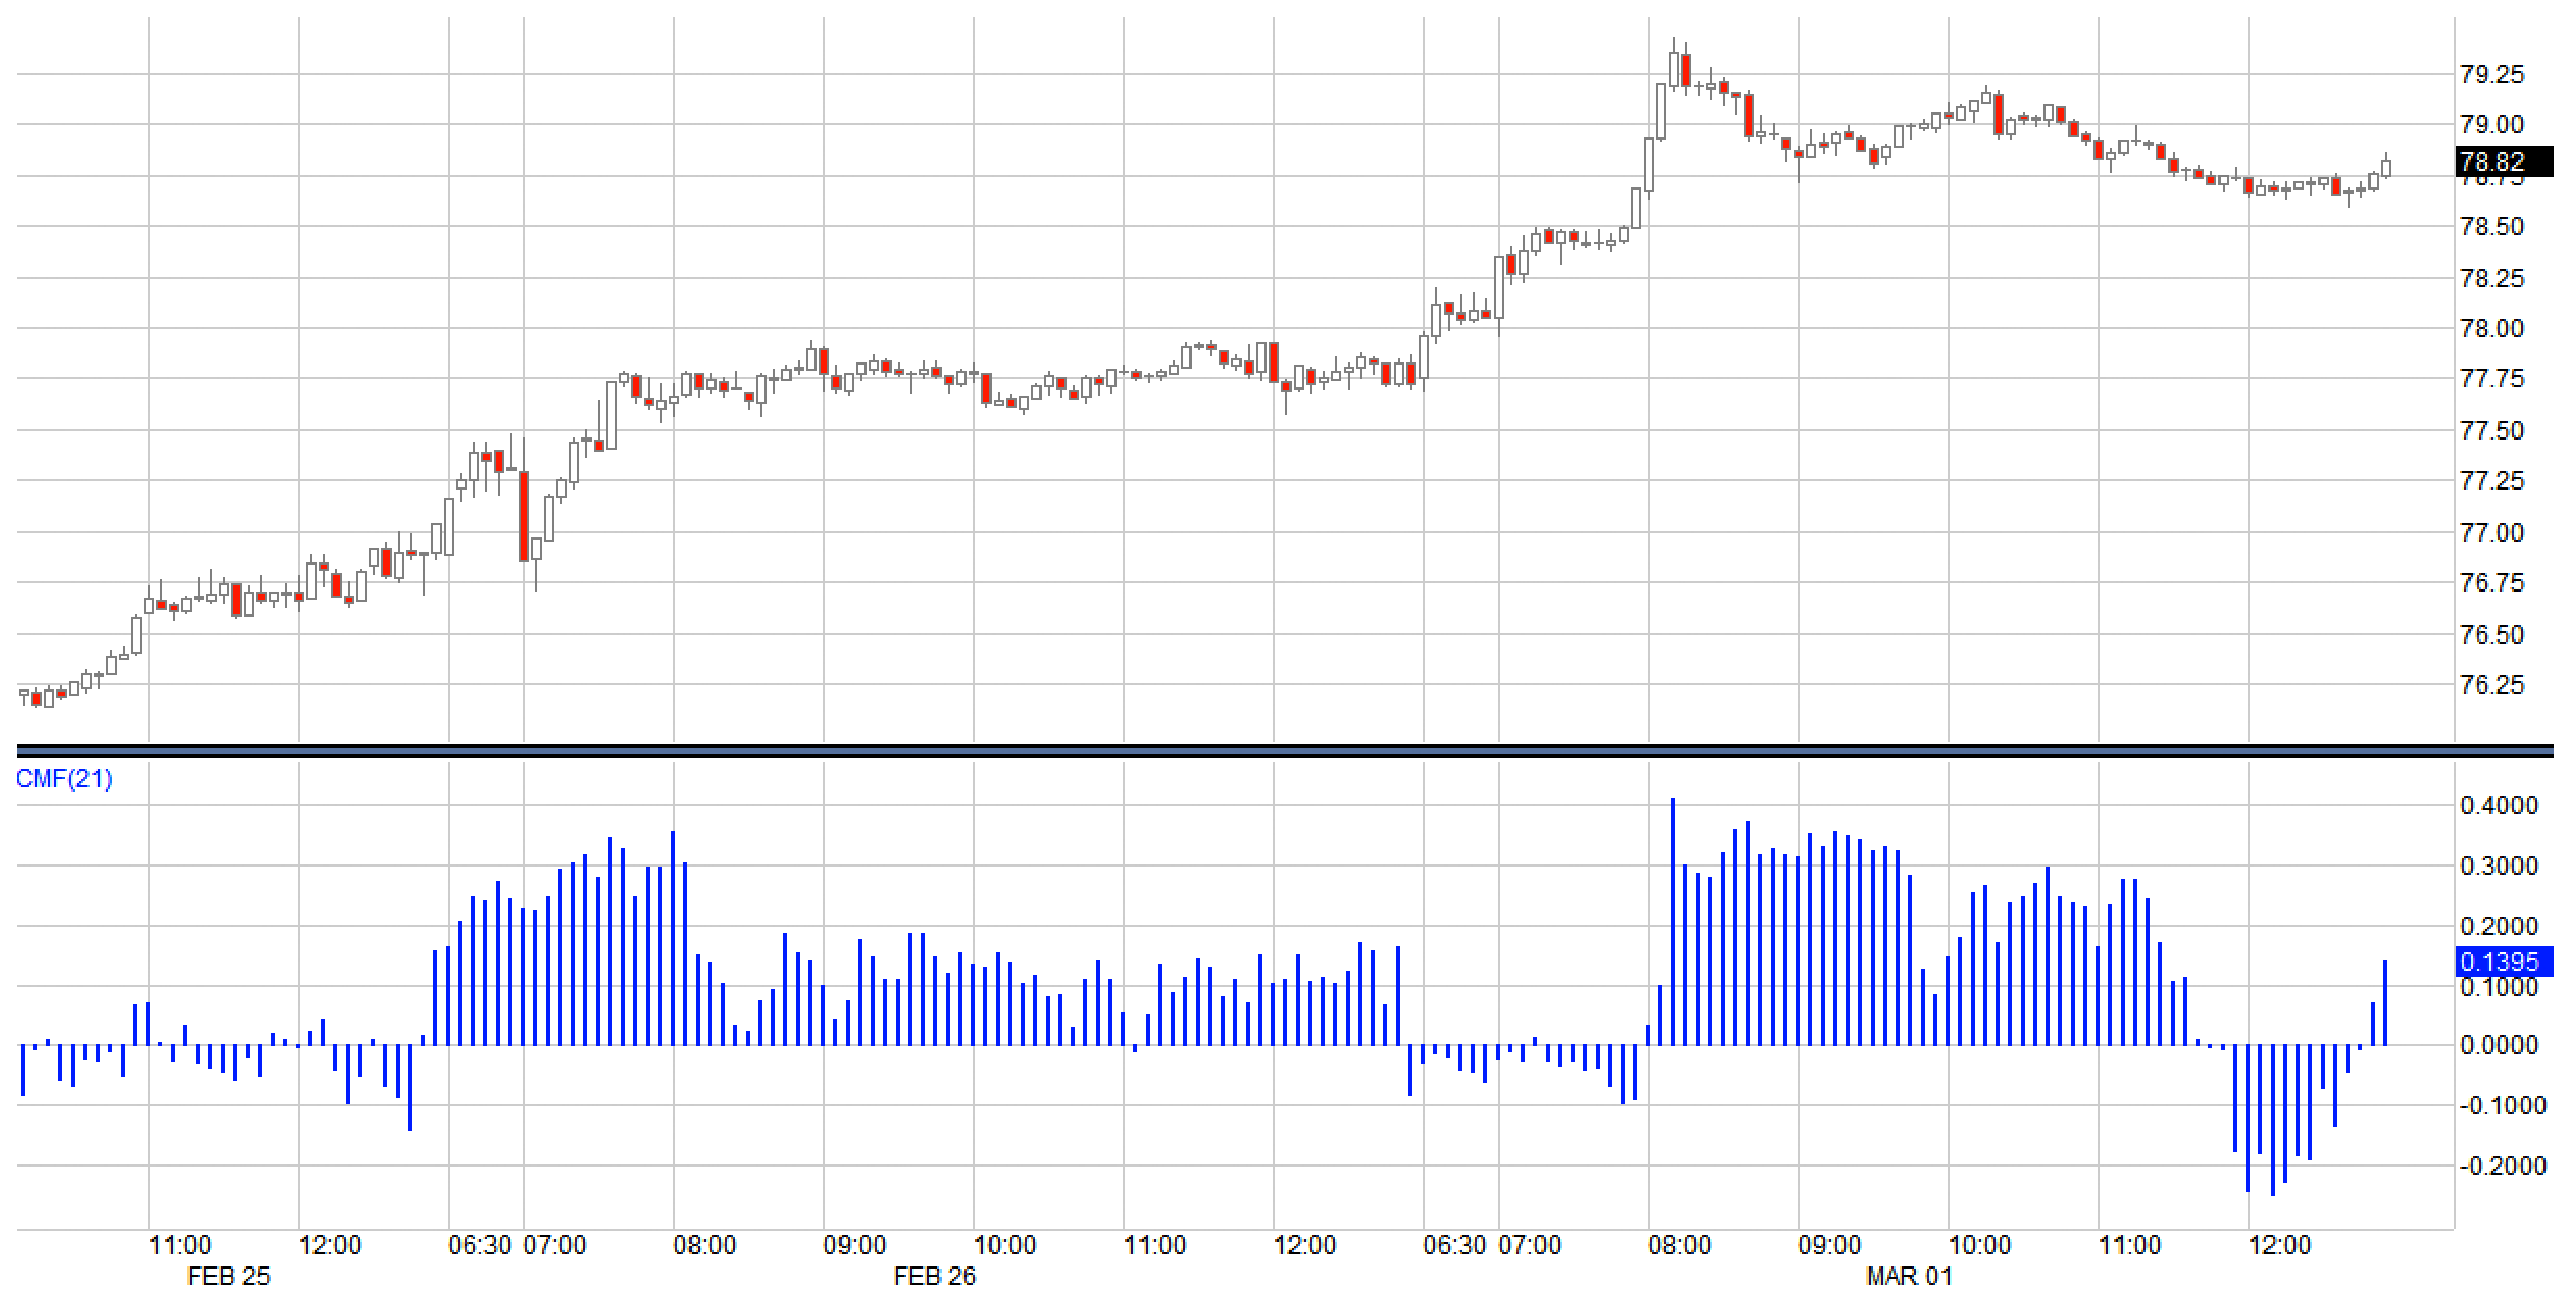
\includegraphics[width=1\textwidth]{figures/CMF-LMT-1.eps}
\caption{$CMF\{c_{LMT \approx 2009}\}$}
\end{figure}

%\section{Relative Strenght Index (RSI)}
%



